\chapter{Marco Teórico}
% ***********************************************************************************

%En linguística existe un esquema de comunicación, llamado \textit{''Esquema de Comunicación de Jakobson''} en el que se enuncian los elementos que forman parte de un proceso de comunicación y que lo conforman; el emisor, el receptor, el código, el mensaje y el canal, los cuales son todos elementos presentes en un proceso de comunicación como el que existen hoy en día, donde hablamos desde actos comunicativos más tradicionales como una nota, una conversación, hasta otros más recientemente instalados en nuestro día a día como lo son el enviar un email, un mensaje de texto, un mensaje por Facebook o Whatsapp. Para que esto sea posible, además de existir un emisor, un receptor y un mensaje, debe existir un canal, y en comunicaciones existen dos categorías que agrupan los tipos de medios, estos pueden ser guiados o no guiados.\\
%
%En el caso de las telecomunicaciones se tiene que el canal de transmisión es el aire, y que por el las ondas electromagnéticas, se propagan sujetas a atenuaciones, reflexiones y refracciones que se producen en las distintas superficies en las que estas inciden.
%%Los medios guiados corresponden a medios de transmisión tales como el cable de par trenzado, cable coaxial o fibra óptica. Mientras en que los medios no guiados son aquellos que utilizan la energía electromagnética que viaja en forma de ondas en un amplio espectro de longitudes de onda, para hacer uso de ella en tecnologías inalámbricas de transmisión de datos en las que se puede encontrar al \ac{WiFi}.\\
%%
%%La tecnología \ac{WiFi} permite la interconexión no cableada de dispositivos electrónicos, permitiendo que estos puedan conectarse a internet a través de un Punto de acceso o \ac{AP}. Este es un dispositivo que opera dentro de lo que el modelo a nivel de la capa física, del modelo OSI.\\

En el proceso de comunicación se tiene que además del emisor, el receptor y el mensaje, existe el canal, el cual para la propagación de las ondas electromagnéticas corresponden al aire o bien, a un cable conductor.\\

Estas son usadas para transmitir información en forma de señales que en comunicaciones, viajan por distintos medios, cables de cobre, fibra óptica o enlaces de microondas, entre otros.\\

Sin embargo, la información, considerando el volumen de datos que viajan por las redes, obedece un orden, que en redes de datos se conoce como modelo OSI.\\

\textbf{Modelo OSI}\\

Es un modelo que sirve de referencia para los protocolos que operan en las distintas capas que componen este modelo. Es un estándar desarrollado en 1980 por la ISO que establece un ordenamiento por el cual deben regirse los datos al moverse.\\

\underline{Este modelo consta de siete capas}\\

Físico, Enlace, Red, Transporte, Sesión, Presentación, Aplicación.

Donde cada nivel realiza una función concreta, y se separa de los adyacentes por interfaces conocidas, sin que le concierna ningún otro aspecto del total de la comunicación.  Las capas que participan de los modelos estudiados son las que se detallan a continuación:

\begin{itemize}

\item{\textbf{Capa Física}

Corresponde a las capa que guarda relación con la conexión, es decir, con la forma en que se conecta el dispositivo a la red y la transmisión, esto es a cómo se transmiten los datos. Entre sus funciones, está el establecer cuál o cuáles son los medios por los cuales viaja la señal y el normar las características materiales y eléctricas de los componentes.\\
}

\item{
\textbf{Capa de Enlace}\\
Esta capa representa para efectos de lo que se pretende investigar y eventualmente desarrollar, la capa que hace posible el seguimiento, pues se encarga de la transferencia de información entre la capa de red y la capa física. Y para ello se vale de tramas que le dotan al dispositivo una dirección \ac{MAC} lo que le permite hacer control de flujo, detección y corrección de errores.\\

Es de esta capa que los IPS, se valen, como es el caso de el algoritmo de trilateración en donde se establece la conexión a un AP, se hace la identificación del dispositivo a través de la dirección MAC y luego el posterior cálculo.\\
}
\end{itemize}

\newpage

\textbf{Medio No Guiado}\\

Corresponde a los medios por los cual viajan las ondas electromagnéticas y que en este caso, corresponden a dispositivos que se valen de antenas para propagarlas.\\

\textbf{Router}

Un router inalámbrico es un dispositivo que además de la función de router, sirve de punto de acceso, es decir, permite que los dispositivos inalámbricos se conecten a la red. En las funciones de router, este dispositivo direcciona los datos que provienen desde y hacia los dispositivos conectados a la red y que compartan la misma conexión de red por las distintas interfaces que la compongan, permitiendo que estos se comuniquen entre sí.\\

Todas las conexiones realizadas en la red inalámbrica se hacen dentro de lo que se denomina, para cuando se usa este tipo de redes, una red de infraestructura inalámbrica y es sobre esta que los dispositivos se comunican entre si e interactúan con la red exterior.\\

Es en esta parte donde el router recibe, desde el dispositivo móvil, solicitudes del tipo \textsc{ICMPV6}, que son un tipo de solicitudes conocidas como \ac{IRDP}  o Protocolo de descubrimiento de enrutador de internet y que son un tipo de solicitudes del protocolo \ac{ICMP} o Protocolo de control de mensajes de internet que se encargan de establecer la conexión con el router. Del tipo de mensajes ICMP existen dos tipos:\\

\begin{itemize}
\item{\textit{ICMP Router Solicitation Message:} Este tipo de mensajes es enviado desde un equipo a cualquiera de los routers que se hallen en la LAN para avisar que se encuentran en presencia de esta red. Básicamente, avisan que podrían eventualmente desear conectarse.}
\item{\textit{ICMP Router Advertisement Message}: Es enviado por el router en la LAN para anunciar la IP disponible para rutear.}\\
\end{itemize}

\begin{figure}[h!]
\centering
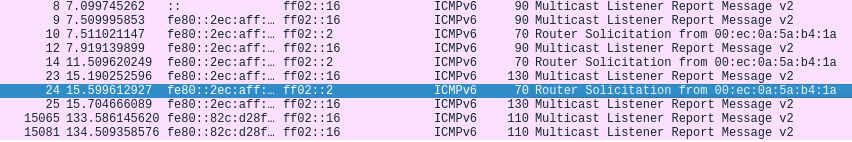
\includegraphics[scale=0.5]{./imagenes/IRDP}
\caption{Captura en Wireshark de solicitudes IRDP}
\label{fig:IRDP}
\end{figure}

Finalmente, se anuncian mediante una solicitud de establecimiento de conexión donde el router recibe la MAC del dispositivo, entre otros datos, y establece la conexión si la autenticación fue existosa.\\


\begin{figure}[h!]
\centering
		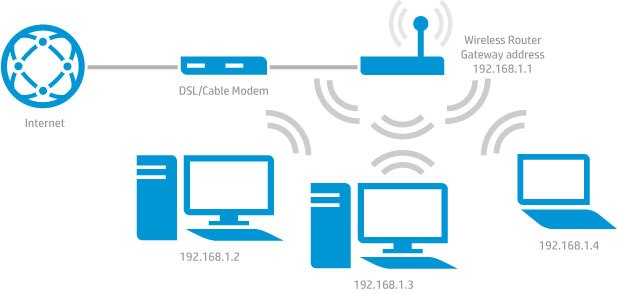
\includegraphics[scale=0.5]{./imagenes/ap}
		\label{fig:access_point}
		\caption{Ejemplo de red de infraestructura inalámbrica$^{\ref{fig:paginaHP}}$}
\end{figure}

De ser exitosa, el router, mediante el protocolo \ac{DHCP}, asigna desde el número limitado de direcciones IP que el \ac{ISP} entrega al cliente, una IP que enlaza esta dirección con la MAC del usuario estableciendo así la conexión. Es así como del router inalámbrico el dispositivo posee ahora la conexión al AP WiFi.\\\\

\textbf{Wifi}\\

Es una tecnología que recibe su nombre a partir de la abreviación de una marca comercial y que permite el acceso a la red por parte de dispositivos de forma inalámbrica, haciendo así posible  la vinculación de diferentes equipos entre si prescindiendo de cables.\\

Dado que la conexión inalámbrica se hace a través de ondas electromagnéticas dentro del rango de frecuencias en los 2.4 GHz y que estas se dividen en 14 canales que van desde los 2412 MHz hasta los 2484 MHz, existen combinaciones óptimas de canales en las que estos no se solapan entre si, y con ello, se logran reducir las interferencias.\\

Esta tecnología está regulada por el estándar internacional IEEE 802.11 que con el paso del tiempo, ha dado lugar a otras versiones que incluyen mejoras tales como ancho de banda, alcance, velocidad y frecuencia.\\

Para efectos de este estudio, se deben tener en consideración las pérdidas propias de la propagación de estas ondas. Ejemplo de la propagación de la señal de Wifi en un espacio es el presentado en la imagen \ref{fig:propagacion} \\

\begin{figure}[h!]
\centering
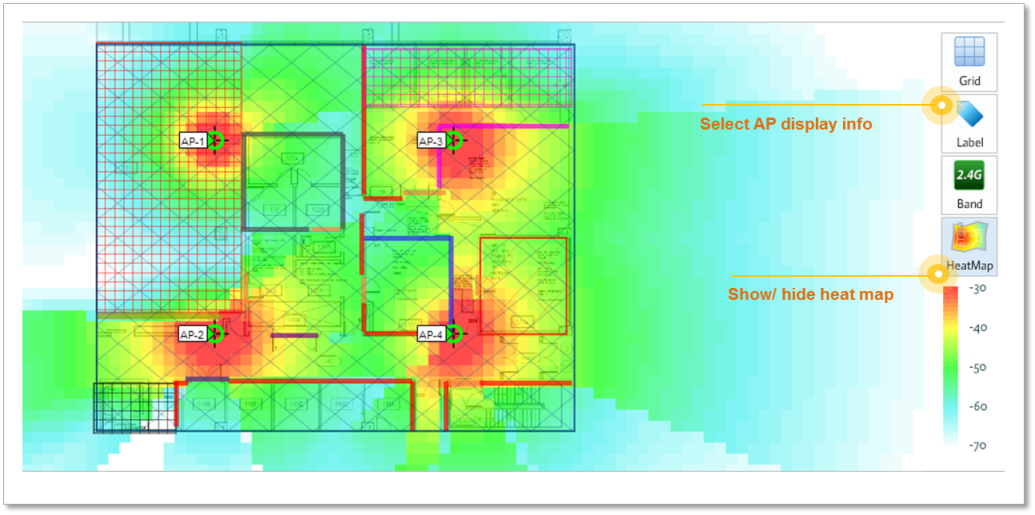
\includegraphics[scale=0.8]{./imagenes/propagacion}
\caption{Muestra software D-link sobre variación de intensidad de señal por propagación en espacio indoor.$^{\ref{fig:prop}}$}
\label{fig:propagacion}
\end{figure}

\newpage 

\textbf{Modelo de propagación}\\

Son aproximaciones matemáticas que permiten modelar el espacio físico por el cual se va a propagar la señal y que contemplan los principios físicos que la describen y que se introducen al modelo en forma de parámetros. Y que para efectos de este estudio, permiten caracterizar los valores esperados según el tipo de espacio que se vaya a caracterizar para así tener un marco de referencia con el cual contrastar las mediciones obtenidas.\\

Se tiene además, 

\begin{itemize}

\item{\textbf{Modelo de propagación Outdoor}
}
\item{
\textbf{Modelo de propagación Indoor}\\

Corresponden a un tipo de modelo de propagación que se adecúa a la forma en que se propagan las ondas en un espacio indoor. Contemplan fenómenos físicos como son la reflexión, la refracción y la atenuación. Estudian además, cuáles son las variantes que se adecúan mejor al espacio, es decir, si se trata de un espacio físico de varios 
pisos o de una sola planta.\\
}
%\textbf{AOA, Angulo de llegada}\\
%
%Tiempo de llegada es el tiempo de viaje entre el transmisor y el receptor. La distancia puede ser usada calculando el tiempo de viaje, por la velocidad de la luz. Para medir el tiempo de viaje en el aire, esta aproximación usualmente requiere sincronización entre transmisores y receptores, para evitar errores de cálculo debido a desfases.\\

%\textbf{TOA, Tiempo de llegada}\\

%En redes de computadoras, ICMP Internet Router Discovery Protocol (IRDP) o Internet Router Discovery Protocol es un protocolo que utiliza mensajes ICMP router advertisement y router solicitudes para permitir a un nodo descubrir la dirección de routers operacionales en una subred IPv4.1​
%
%Este protocolo es utilizado en IP móvil para cuando un nodo móvil se encuentra cambiando constantemente de subred sin tener que perder comunicación con su "Home Agent" (HA).

\end{itemize}